\begin{figure}
\centering
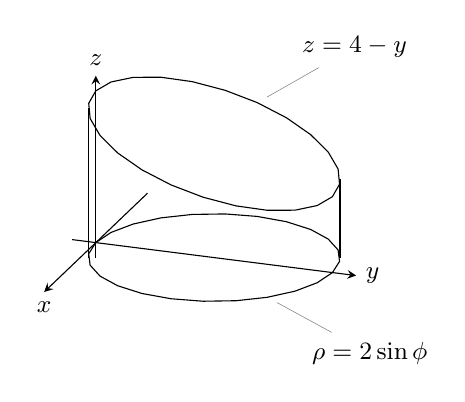
\begin{tikzpicture}[font=\small,declare function={fx(\t)=cos(\t);fy(\t)=1+sin(\t);fz(\t)=4-1-sin(\t);}]
\pgfmathsetmacro{\kx}{0.35}
\pgfmathsetmacro{\ky}{\kx^2}
\pgfmathsetmacro{\kz}{1-\ky}
\pgfmathsetmacro{\tp}{110}
\pgfmathsetmacro{\tpa}{180+\tp}
\begin{axis}[clip=false,view/h=110,small,axis lines=middle,xtick={\empty},ytick={\empty},ztick={\empty},enlargelimits=true, xlabel={$x$}, ylabel={$y$},zlabel={$z$}, xlabel style={anchor=north},ylabel style={anchor=west},zlabel style={anchor=south},colormap={}{gray(0cm)=(0.6);gray(1cm)=(0.9);}]
\addplot3[black,domain=0:360,variable=\t]({fx(t)},{fy(t)},{0})node[pos=0.125,pin=-45:{$\rho=2\sin\phi$}]{};
\addplot3[black,domain=0:360,variable=\t]({fx(t)},{fy(t)},{fz(t)})node[pos=0.5,pin=45:{$z=4-y$}]{};
\addplot3[]plot coordinates {({fx(\tp)},{fy(\tp)},{0})({fx(\tp)},{fy(\tp)},{fz(\tp)})};
\addplot3[]plot coordinates {({fx(\tpa)},{fy(\tpa)},{0})({fx(\tpa)},{fy(\tpa)},{fz(\tpa)})};
\end{axis}
\end{tikzpicture}
\end{figure}


\begin{figure}
\centering
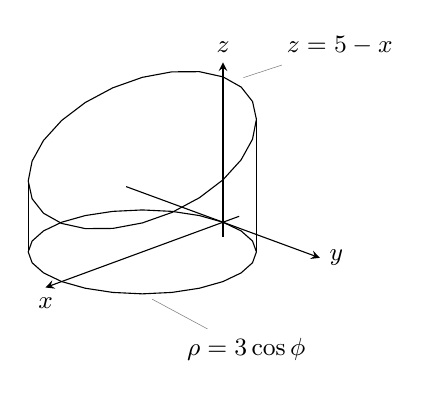
\begin{tikzpicture}[font=\small,declare function={fx(\t)=3/2+3/2*cos(\t);fy(\t)=3/2*sin(\t);fz(\t)=5-3/2-3/2*cos(\t);}]
\pgfmathsetmacro{\kx}{0.35}
\pgfmathsetmacro{\ky}{\kx^2}
\pgfmathsetmacro{\kz}{1-\ky}
\pgfmathsetmacro{\tp}{135}
\pgfmathsetmacro{\tpa}{180+\tp}
\begin{axis}[clip=false,view/h=135,small,axis lines=middle,xtick={\empty},ytick={\empty},ztick={\empty},enlargelimits=true, xlabel={$x$}, ylabel={$y$},zlabel={$z$}, xlabel style={anchor=north},ylabel style={anchor=west},zlabel style={anchor=south},colormap={}{gray(0cm)=(0.6);gray(1cm)=(0.9);}]
\addplot3[black,domain=0:360,variable=\t]({fx(t)},{fy(t)},{0})node[pos=0.125,pin=-45:{$\rho=3\cos\phi$}]{};
\addplot3[black,domain=0:360,variable=\t]({fx(t)},{fy(t)},{fz(t)});
\addplot3[]plot coordinates {(0,0.2,5)}node[pin=20:{$z=5-x$}]{};
\addplot3[]plot coordinates {({fx(\tp)},{fy(\tp)},{0})({fx(\tp)},{fy(\tp)},{fz(\tp)})};
\addplot3[]plot coordinates {({fx(\tpa)},{fy(\tpa)},{0})({fx(\tpa)},{fy(\tpa)},{fz(\tpa)})};
\end{axis}
\end{tikzpicture}
\end{figure}


\begin{figure}
\centering
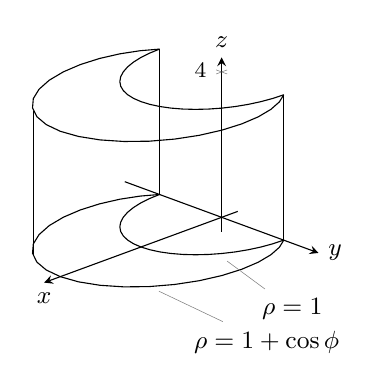
\begin{tikzpicture}[font=\small,declare function={fr(\t)=1+cos(\t);gr(\t)=1;fy(\t)=3/2*sin(\t);fz(\t)=5-3/2-3/2*cos(\t);}]
\pgfmathsetmacro{\kx}{0.35}
\pgfmathsetmacro{\ky}{\kx^2}
\pgfmathsetmacro{\kz}{1-\ky}
\pgfmathsetmacro{\tp}{90}
\pgfmathsetmacro{\tpa}{-90}
\pgfmathsetmacro{\tpb}{340}
\pgfmathsetmacro{\tpc}{50}
\pgfmathsetmacro{\tpd}{30}
\begin{axis}[clip=false,view/h=135,small,axis lines=middle,xtick={\empty},ytick={\empty},ztick={4},enlargelimits=true, xlabel={$x$}, ylabel={$y$},zlabel={$z$}, xlabel style={anchor=north},ylabel style={anchor=west},zlabel style={anchor=south},colormap={}{gray(0cm)=(0.6);gray(1cm)=(0.9);}]
\addplot3[data cs=polar,domain=-90:90,variable=\t,samples y=0]({t},{fr(t)},{0});
\addplot3[data cs=polar,domain=-90:90,variable=\t,samples y=0]({t},{gr(t)},{0});
\addplot3[data cs=polar,domain=-90:90,variable=\t,samples y=0]({t},{fr(t)},{4});
\addplot3[data cs=polar,domain=-90:90,variable=\t,samples y=0]({t},{gr(t)},{4});
\addplot3[data cs=polar]plot coordinates {({\tp},{fr(\tp)},{0})({\tp},{fr(\tp)},{4})};
\addplot3[data cs=polar]plot coordinates {({\tpa},{fr(\tpa)},{0})({\tpa},{fr(\tpa)},{4})};
\addplot3[data cs=polar]plot coordinates {({\tpb},{fr(\tpb)},{0})({\tpb},{fr(\tpb)},{4})};
\addplot3[data cs=polar,]plot coordinates {({\tpc},{gr(\tpc)},{0})}node[pin=-45:{$\rho=1$}]{};
\addplot3[data cs=polar,]plot coordinates {({\tpd},{fr(\tpd)},{0})}node[pin=-45:{$\rho=1+\cos\phi$}]{};
\end{axis}
\end{tikzpicture}
\end{figure}

